
\begin{figure}[ht]
  \centering
  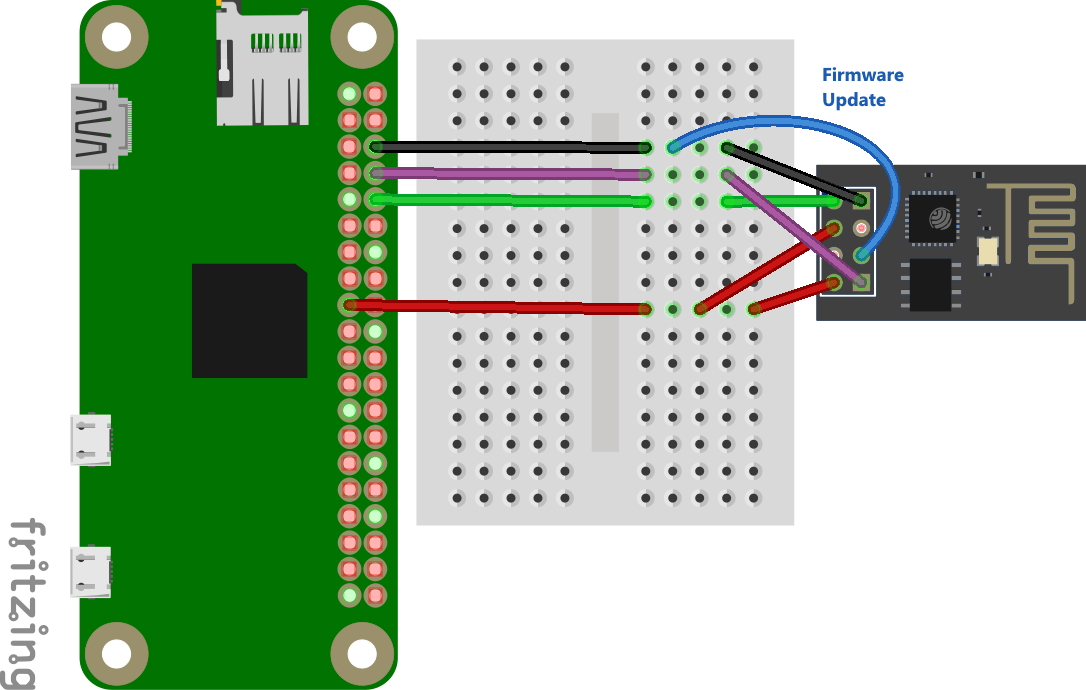
\includegraphics[scale=0.25]{images/ESP8266_ESP-01.png}	
  \ \ \  
  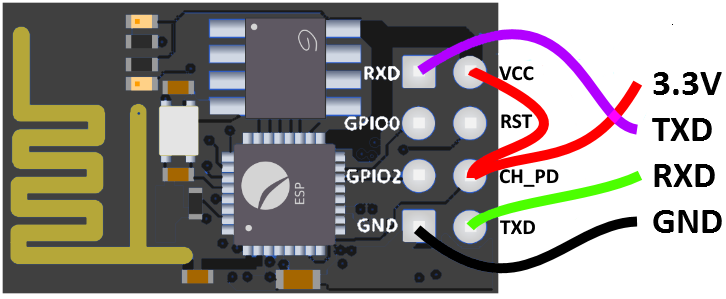
\includegraphics[scale=0.2]{images/ESP8266.png}
  %	\caption{}
  \label{ESP8266_ESP-01}
\end{figure}

\subsection{Firmware Update}

Tools: \url{http://www.espressif.com/en/support/download/other-tools}\\
SDKs und Demos: \url{http://www.espressif.com/en/support/download/sdks-demos}\\
NONOS SDK Source: \url{https://github.com/espressif/ESP8266_NONOS_SDK/releases}\\
Download SDK: \url{https://github.com/espressif/ESP8266_NONOS_SDK/archive/v2.2.1.zip}\\


Um das Firmware Update ausf�hren zu k�nnen muss der GPIO0 Eingang auf GND gesetzt werden. Das kann entweder dauerhaft gemacht werden indem der Pin direkt auf GND verbunden wird. Oder man macht es �ber einen Schalter. Dann ist wichtig, dass der Schalter w�hrend des Boot-Vorgangs bzw. bevor Reset gedr�ckt wird, gedr�ckt gehalten wird. Ich w�rde aber empfehlen einfach den GPIO0 Pin �ber eine Kabel auf GND zu verbinden. Reset kann ausgel�st werden durch entfernen und zur�ckstecken der 3,3~V Versorgung.

Beim schwarzen ESP-01 (1~MBit) m�ssen folgende Dateien und Adressen �bertragen werden.    

\begin{table}[h]
\caption{ Schwarzer ESP01 (1~MBit) Firmware Dateien}
\centering
\begin{tabular}{|l|c|c|}
\hline
\textbf{Datei (NONOS SDK)} & \textbf{Adresse} \\
\hline
\path{bin/blank.bin} & 0xFB000\\
\hline
\path{bin/esp_init_data_default_v08.bin} & 0xFC000\\
\hline
\path{bin/blank.bin} & 0x7E000\\
\hline
\path{bin/blank.bin} & 0xFE000\\
\hline
\path{bin/boot_v1.7.bin} & 0x00000\\
\hline
\path{bin/at/512+512/user1.1024.new.2.bin} & 0x01000\\
\hline
\end{tabular}
\end{table}



\subsubsection{Linux (Raspberry Pi)}

\begin{console}
cd ~
wget https://github.com/espressif/ESP8266_NONOS_SDK/archive/v2.1.0.zip
unzip v2.1.0.zip
sudo apt-get install python python-pip
sudo pip install esptool
\end{console}

%pip2 install esptool


\begin{console}
esptool.py version
\end{console}

\begin{screensmall}
esptool.py v2.1
2.1
\end{screensmall}

\begin{console}
python esptool.py -p /dev/ttyAMA0 flash_id 
\end{console}


%ttyUSB0 
\begin{console}
cd ESP8266_NONOS_SDK-2.1.0/bin/
sudo esptool.py -p /dev/ttyAMA0 write_flash 0x00000 boot_v1.6.bin 0x01000 at/512+512/user1.1024.new.2.bin \
 0xFB000 blank.bin 0xFC000 esp_init_data_default.bin 0x7E000 blank.bin 0xFE000 blank.bin 
\end{console}



%
\subsubsection{Windows}


Download Flash Tool: \url{http://www.espressif.com/sites/default/files/tools/flash_download_tools_v3.4.9.2_0.zip}\\

Nach dem Download des letzten Release des NONOS SDK und des Flash Tool m�ssen beide Archive entpackt werden.
Dann kann das Flash Tool "`ESPFlashDownloadTool\_v3.4.9.2.exe"' gestartet werden. Nun  muss die korrekte COM-Nummer ausgew�hlt und die Bautrate auf 115200 gestellt werden. Danach kann mit der Start Taste der ESP gesucht werden. Wenn dies erfolgreich ist werden verschiedene Daten der Platine ausgelesen und im Fenster angezeigt.\\
Dann k�nnen die verschienden Dateien der neuen Firmware aus dem "`bin"' Verzeichnis des NONOS SDKs ausgew�hlt werden. Zu jeder Datei muss noch eine Start-Adresse eingeben werden.\\
Beim ESP-01 (8~MBit) m�ssen die angegebenen Dateien und Adressen eingegeben und �bertragen werden.    

\begin{figure}[ht]
  \centering
  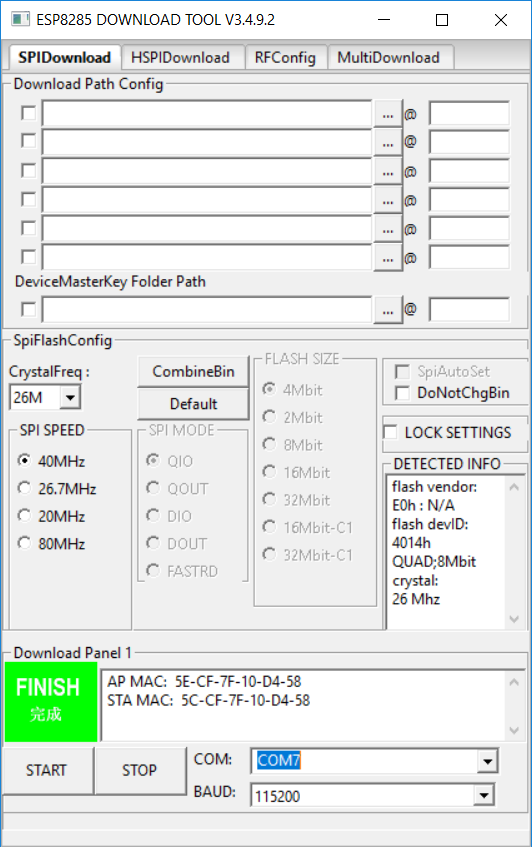
\includegraphics[scale=1.00]{images/ESP8266-ESP_01_FW_update_1.png}	
  %	\caption{}
  \label{ESP8266_ESP-01_FW_UPDATE_1}
\end{figure}

Danach kann mit der Start Taste die Aktualisierung gestartet werden. Wenn der blaue Balken das Ende erreicht hat, kann der ESP aus- und wieder angesteckt werden. Nun sollte die neue Firmware aktiv sein. Mit einem Terminalprogramm wie Putty (COM Verbindung) kann die Version abgefragt werden.

\begin{figure}[ht]
  \centering
  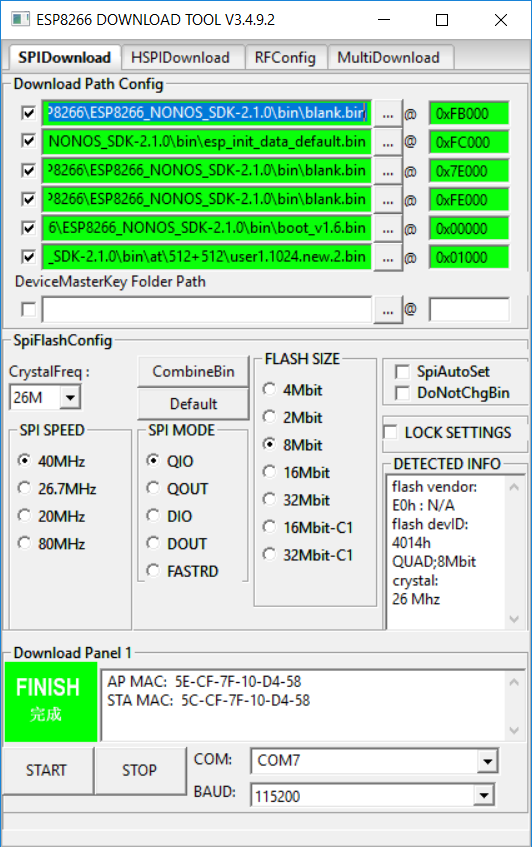
\includegraphics[scale=1.00]{images/ESP8266-ESP_01_FW_update_2.png}	
  %	\caption{}
  \label{ESP8266_ESP-01_FW_UPDATE_2}
\end{figure}


\begin{figure}[ht]
  \centering
  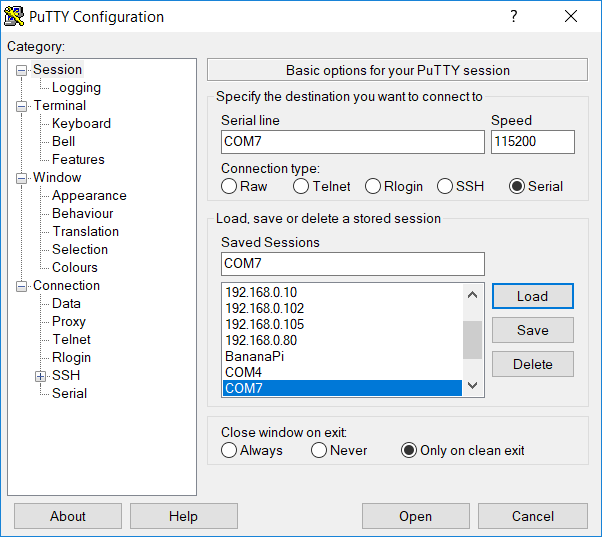
\includegraphics[scale=1.00]{images/Putty_COM.png}	
  %	\caption{}
  \label{Putty_COM}
\end{figure}

\begin{console}
Version abfragen: AT+GMR
\end{console}
\framebox{Enter} \framebox{Strg}+\framebox{J} 


\begin{screensmall}
AT version:1.4.0.0(May  5 2017 16:10:59)
SDK version:2.1.0(116b762)
compile time:May  5 2017 16:37:48
OK
\end{screensmall}



\subsection{Verwendung}


\textbf{AT-Befehlsatz:}\\
\url{https://www.espressif.com/sites/default/files/documentation/4a-esp8266_at_instruction_set_en.pdf}\\


\begin{figure}[ht]
  \centering
  
\includegraphics[scale=0.18]{images/QR_ESP8266_AT-Cmd.png}	
  %	\caption{}
  \label{ESP8266_AT-Cmd}
\end{figure}

Vor dem Verbindungsaufbau muss zuerst der serielle Terminal beendet werden. Bei GC2-xHAT kann dies mit dem Befehl "`esppoweron"' erledigt werden. Dieser schaltet danach die Versorgung des ESP-Moduls ein. Dann kann �ber das Programm screen mit dem Mikrocontroller kommuniziert werden. Alle Befehle m�ssen allerdings mit Enter und STRG+J abgeschlossen werden. 
%\textbf{Raspberry Pi:}
\begin{console}
sudo systemctl stop serial-getty@ttyAMA0.service
sudo systemctl status serial-getty@ttyAMA0.service
\end{console}
%sudo apt-get install screen


\begin{console}
sudo screen /dev/ttyAMA0 115200
\end{console}

%\textbf{USB UART:} 
%\begin{console}
%sudo screen /dev/ttyUSB0 115200
%\end{console}

%\textbf{Beispielkommunikation:}

\textbf{Verbindungstest:} \texttt{AT} \framebox{Enter} \framebox{Strg}+\framebox{J} 
\begin{screensmall}
OK
\end{screensmall}

\textbf{Reset:} \texttt{AT+RST} \framebox{Enter} \framebox{Strg}+\framebox{J}
\begin{screensmall}
2nd boot version : 1.7(5d6f877)
SPI Speed : 40MHz
SPI Mode : QIO
SPI Flash Size & Map: 8Mbit(512KB+512KB)
jump to run user1 @ 1000
\end{screensmall}


% Updated ESP-01


% ets Jan  8 2013,rst cause:2, boot mode:(3,6)
% 
% load 0x40100000, len 1396, room 16
% tail 4
% chksum 0x89
% load 0x3ffe8000, len 776, room 4
% tail 4
% chksum 0xe8
% load 0x3ffe8308, len 540, room 4
% tail 8
% chksum 0xc0
% csum 0xc0
% 
% 2nd boot version : 1.4(b1)
% SPI Speed      : 40MHz
% SPI Mode       : DIO
% SPI Flash Size & Map: 8Mbit(512KB+512KB)
% jump to run user1 @ 1000
% 
% Ai-Thinker Technology Co.,Ltd.

% ets Jan  8 2013,rst cause:2, boot mode:(3,7)
% 
% load 0x40100000, len 1856, room 16 
% tail 0
% chksum 0x63
% load 0x3ffe8000, len 776, room 8 
% tail 0
% chksum 0x02
% load 0x3ffe8310, len 552, room 8 
% tail 0
% chksum 0x79
% csum 0x79
% 
% 2nd boot version : 1.5
% SPI Speed      : 40MHz
% SPI Mode       : DIO
% SPI Flash Size & Map: 8Mbit(512KB+512KB)
% jump to run user1 @ 1000


\textbf{Version abfragen:} \texttt{AT+GMR} \framebox{Enter} \framebox{Strg}+\framebox{J}
\begin{screensmall}
AT version:1.6.2.0(Apr 13 2018 11:10:59)
SDK version:2.2.1(6ab97e9)
compile time:Jun  7 2018 19:34:26
Bin version(Wroom 02):1.6.2
OK
\end{screensmall}


% Updated ESP-01

%AT version:0.40.0.0(Aug  8 2015 14:45:58)
%SDK version:1.3.0
%Ai-Thinker Technology Co.,Ltd.
%Build:1.3.0.2 Sep 11 2015 11:48:04

%AT version:1.1.0.0(May 11 2016 18:09:56)
%SDK version:1.5.4(baaeaebb)
%Ai-Thinker Technology Co. Ltd.
%Jun 13 2016 11:29:20


\textbf{WLAN Modus Station setzen:} \texttt{AT+CWMODE=1} \framebox{Enter} \framebox{Strg}+\framebox{J}
\begin{screensmall}
OK
\end{screensmall}

\textbf{Gefundene WLAN-Netze auflisten:} \texttt{AT+CWLAP} \framebox{Enter} \framebox{Strg}+\framebox{J}
\begin{screensmall}
+CWLAP:(4,"Home",-92,"f4:06:8d:3b:e1:3c",11,-41)
+CWLAP:(3,"AndroidAP",-89,"10:a5:d0:73:de:eb",11,23)
\end{screensmall}


\textbf{LED schalten (nur bei ESP-01S):} \\
\texttt{AT+SYSIOSETCFG=2,0,1} \framebox{Enter} \framebox{Strg}+\framebox{J}\\
\texttt{AT+SYSGPIODIR=2,1} \framebox{Enter} \framebox{Strg}+\framebox{J}\\
\texttt{AT+SYSGPIOWRITE=2,1} \framebox{Enter} \framebox{Strg}+\framebox{J}\\
\texttt{AT+SYSGPIOWRITE=2,0} \framebox{Enter} \framebox{Strg}+\framebox{J}\\
\texttt{AT+SYSGPIODIR=2,0} \framebox{Enter} \framebox{Strg}+\framebox{J}\\

\textbf{Screen beenden:}\\
\framebox{Strg}+\framebox{A} und "`:quit"' eingeben